\section{Submission Flow}
\label{sec:design_flow}

Tiny Tapeout designs are primarily developed in the Verilog hardware description language (HDL) or Wokwi~\cite{wokwi}
Wokwi is a web based visual schematic editor for hardware description, designed as an easier way for individuals with no prior HDL experience to get started.
The Tiny Tapeout website~\cite{tinytapeout} includes a basic getting started guide for Wokwi, demonstrating how to use the tool to draw circuits, which is made available in English and Spanish.

The process of designing an ASIC for submission to Tiny Tapeout, whether with Wokwi, Verilog, or another HDL, matches existing workflows built around the same tools and is outside the scope of this article; instead, we focus here on the aspects of the submission flow which differ from traditional ASIC design and production flows.

\begin{figure}[!t]
\centering
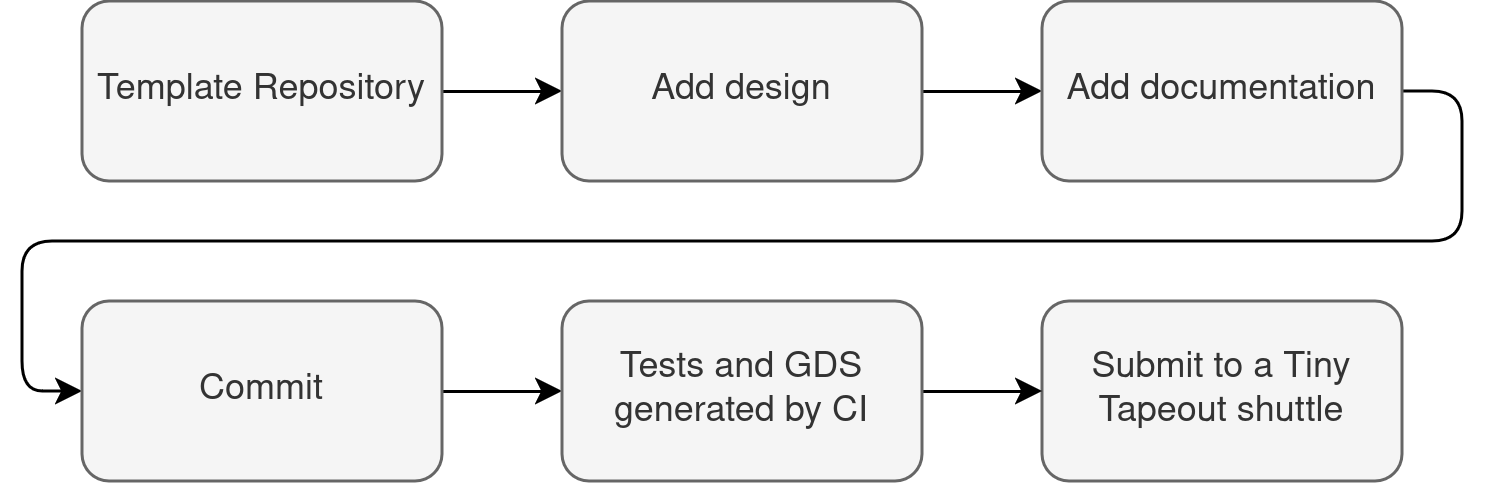
\includegraphics[width=\columnwidth]{./Figs/submission_flow.png}
\caption{Design Submission Flow}
\label{fig:submission_flow}
\end{figure}

The submission flow starts with the participant creating a GitHub~\cite{github} source code repository from a template provided by Tiny Tapeout. Using this template and guidance provided through the Tiny Tapeout website and broader communication channels the participant then creates their chip design in Verilog, Wokwi, or the HDL of their choice.

The participant's design must then be documented, after which the design and its documentation can be commited and pushed to the GitHub repository. This submission triggers automated tests and the generation of binary layout files in GDSII~\cite{gds} format.

This automated testing and GDS generation is handled through the Tiny Tapeout GitHub templates\cite{verilogtemplate} using GitHub Actions\cite{githubactions}---an automatic continuous integration system triggered every time the repository is updated. This reduces duplicated effort and makes it possible for Tiny Tapeout to support large numbers of participants without excessive technical overhead.

There are four main jobs in the continuous integration system:

\begin{enumerate}
	\item GDS: installs OpenLane\cite{openlane} and the SkyWater Sky130\cite{skywaterpdk} PDK, builds the binary layout files, and generates a summary of the design (Fig.~\ref{fig:summary_table_GDS_job}). The summary includes utilization, standard cells used, a 2-D render (Fig.~\ref{fig:render_cells_in_use}) and an interactive 3-D viewer (Fig.~\ref{fig:interactive_3D_viewer}).
This job can also optionally run a gate-level verification of the design.
	\item Verification: installs the YosysHQ open source computer-aided design (CAD) suite, which includes many common electronic design automation (EDA) tools; uses iVerilog\cite{iverilog} and cocotb\cite{cocotb} to run any included testbenches.
	\item Documentation: generates a preview of the documentation.
	\item Precheck: runs design rule check (DRC) tests to ensure the design can be integrated into the multi project chip.
\end{enumerate}

Successful GDS, Documentation, and Precheck job completion are all required for a design to be submitted to a shuttle for production.
Verification is optional but highly encouraged. Submissions designed in Wokwi are able to make use of its integrated truth table testing system\cite{automatedtesting}.

If all tests pass and the binary layout files are correctly generated the design can then be submitted to a quarterly shuttle for production in silicon, alongside all other passing designs from participants in that Tiny Tapeout run. Projects are submitted to a shuttle through the Tiny Tapeout website~\cite{tinytapeout}. Participants are free to update submitted projects up until the closing date of the shuttle, providing the tests continue to pass.

While the Tiny Tapeout continuous integration system can be run entirely in the user's web browser, it is also possible to install a local copy of the tools\cite{localinstall} on a participant's computer. Locally installed tools can help to reduce the time between design iterations, especially for the test and verification jobs.

With its focus on automated testing Tiny Tapeout is able to minimize design errors common to those coming to ASIC design with little or nor prior experience, reducing wastage at the production stage and maximizing

\begin{figure}[!t]
\centering
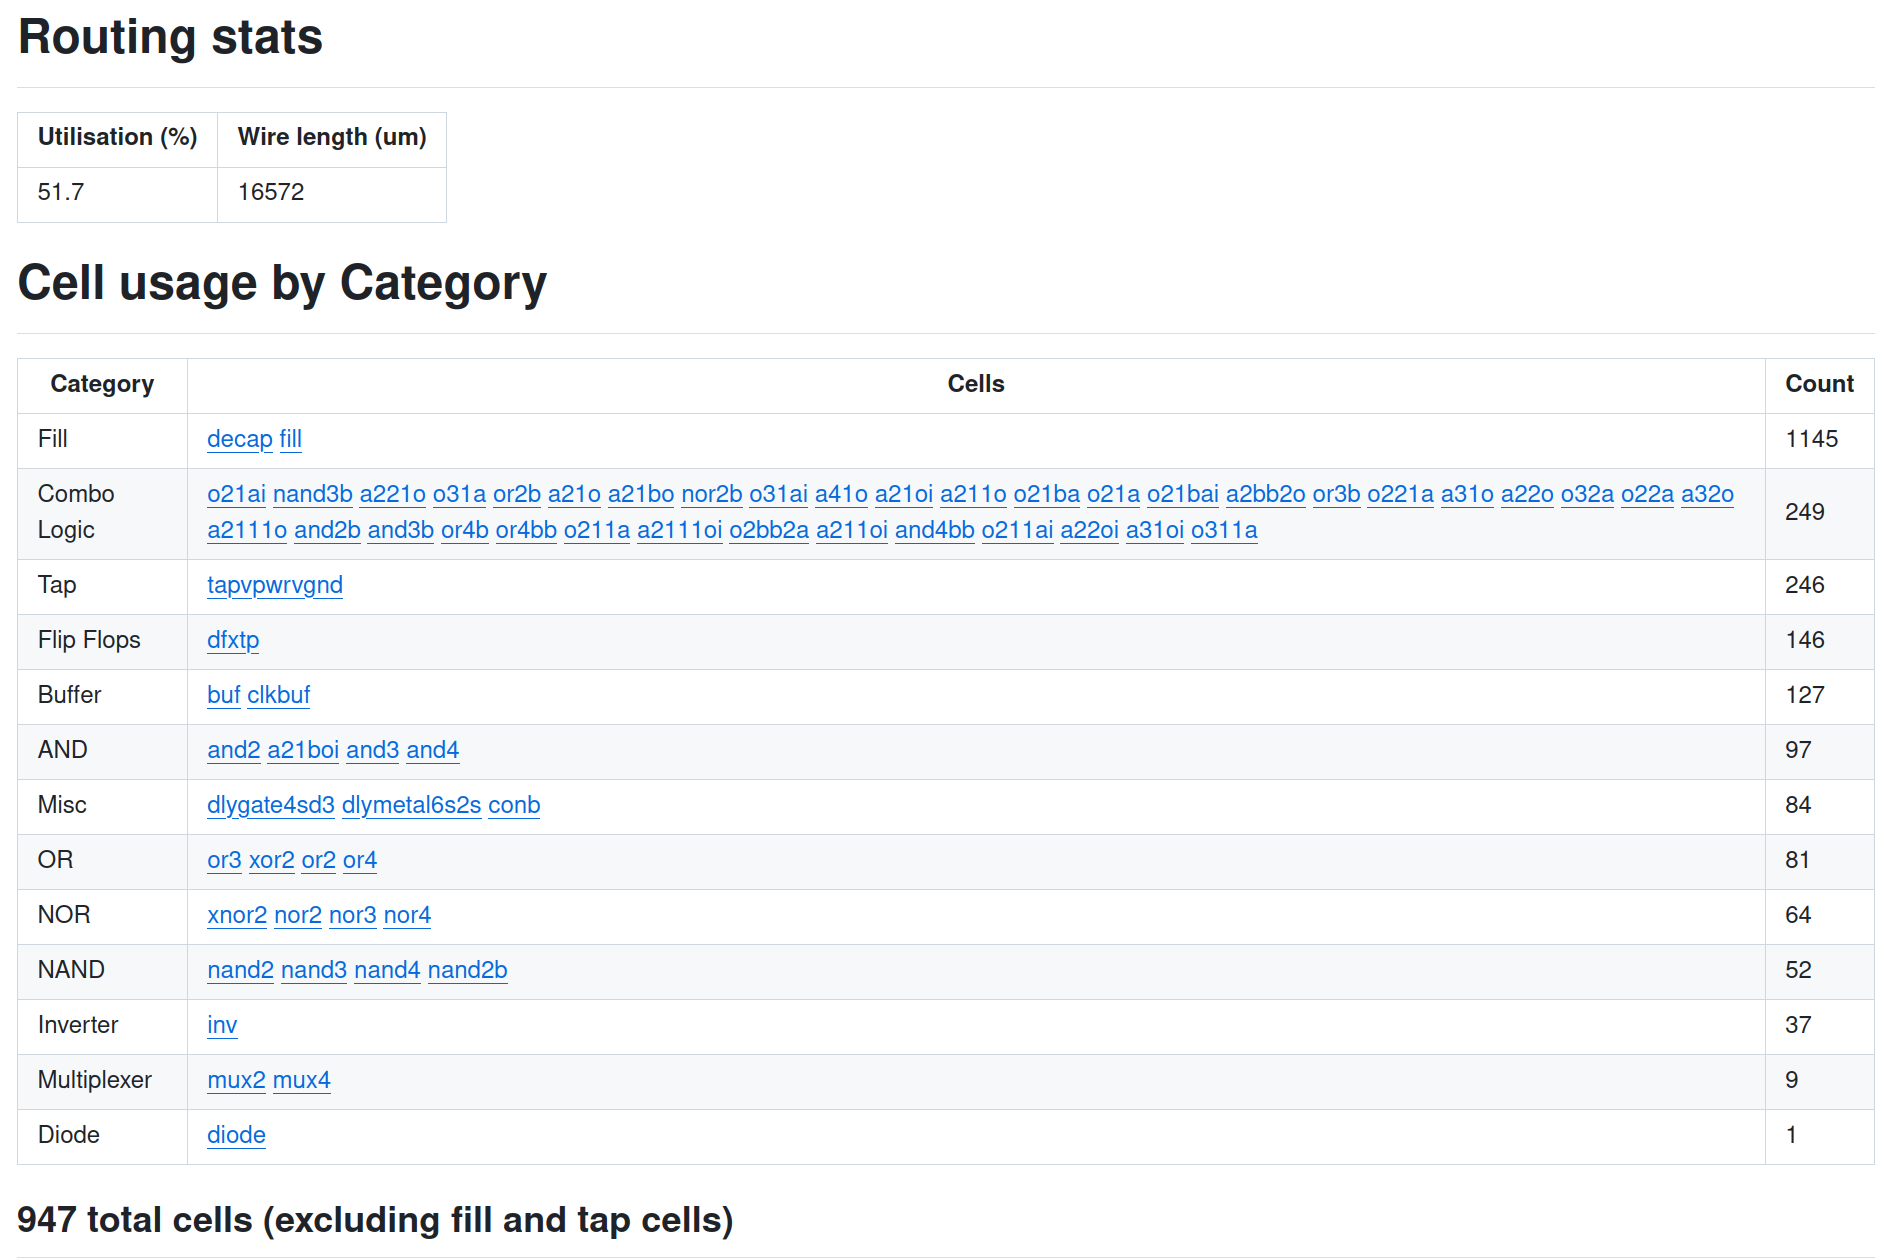
\includegraphics[width=\columnwidth]{./Figs/gh action cell stats.png}
\caption{A summary table from the GDS continuous integration job.}
\label{fig:summary_table_GDS_job}
\end{figure}

\begin{figure}[!t]
\centering
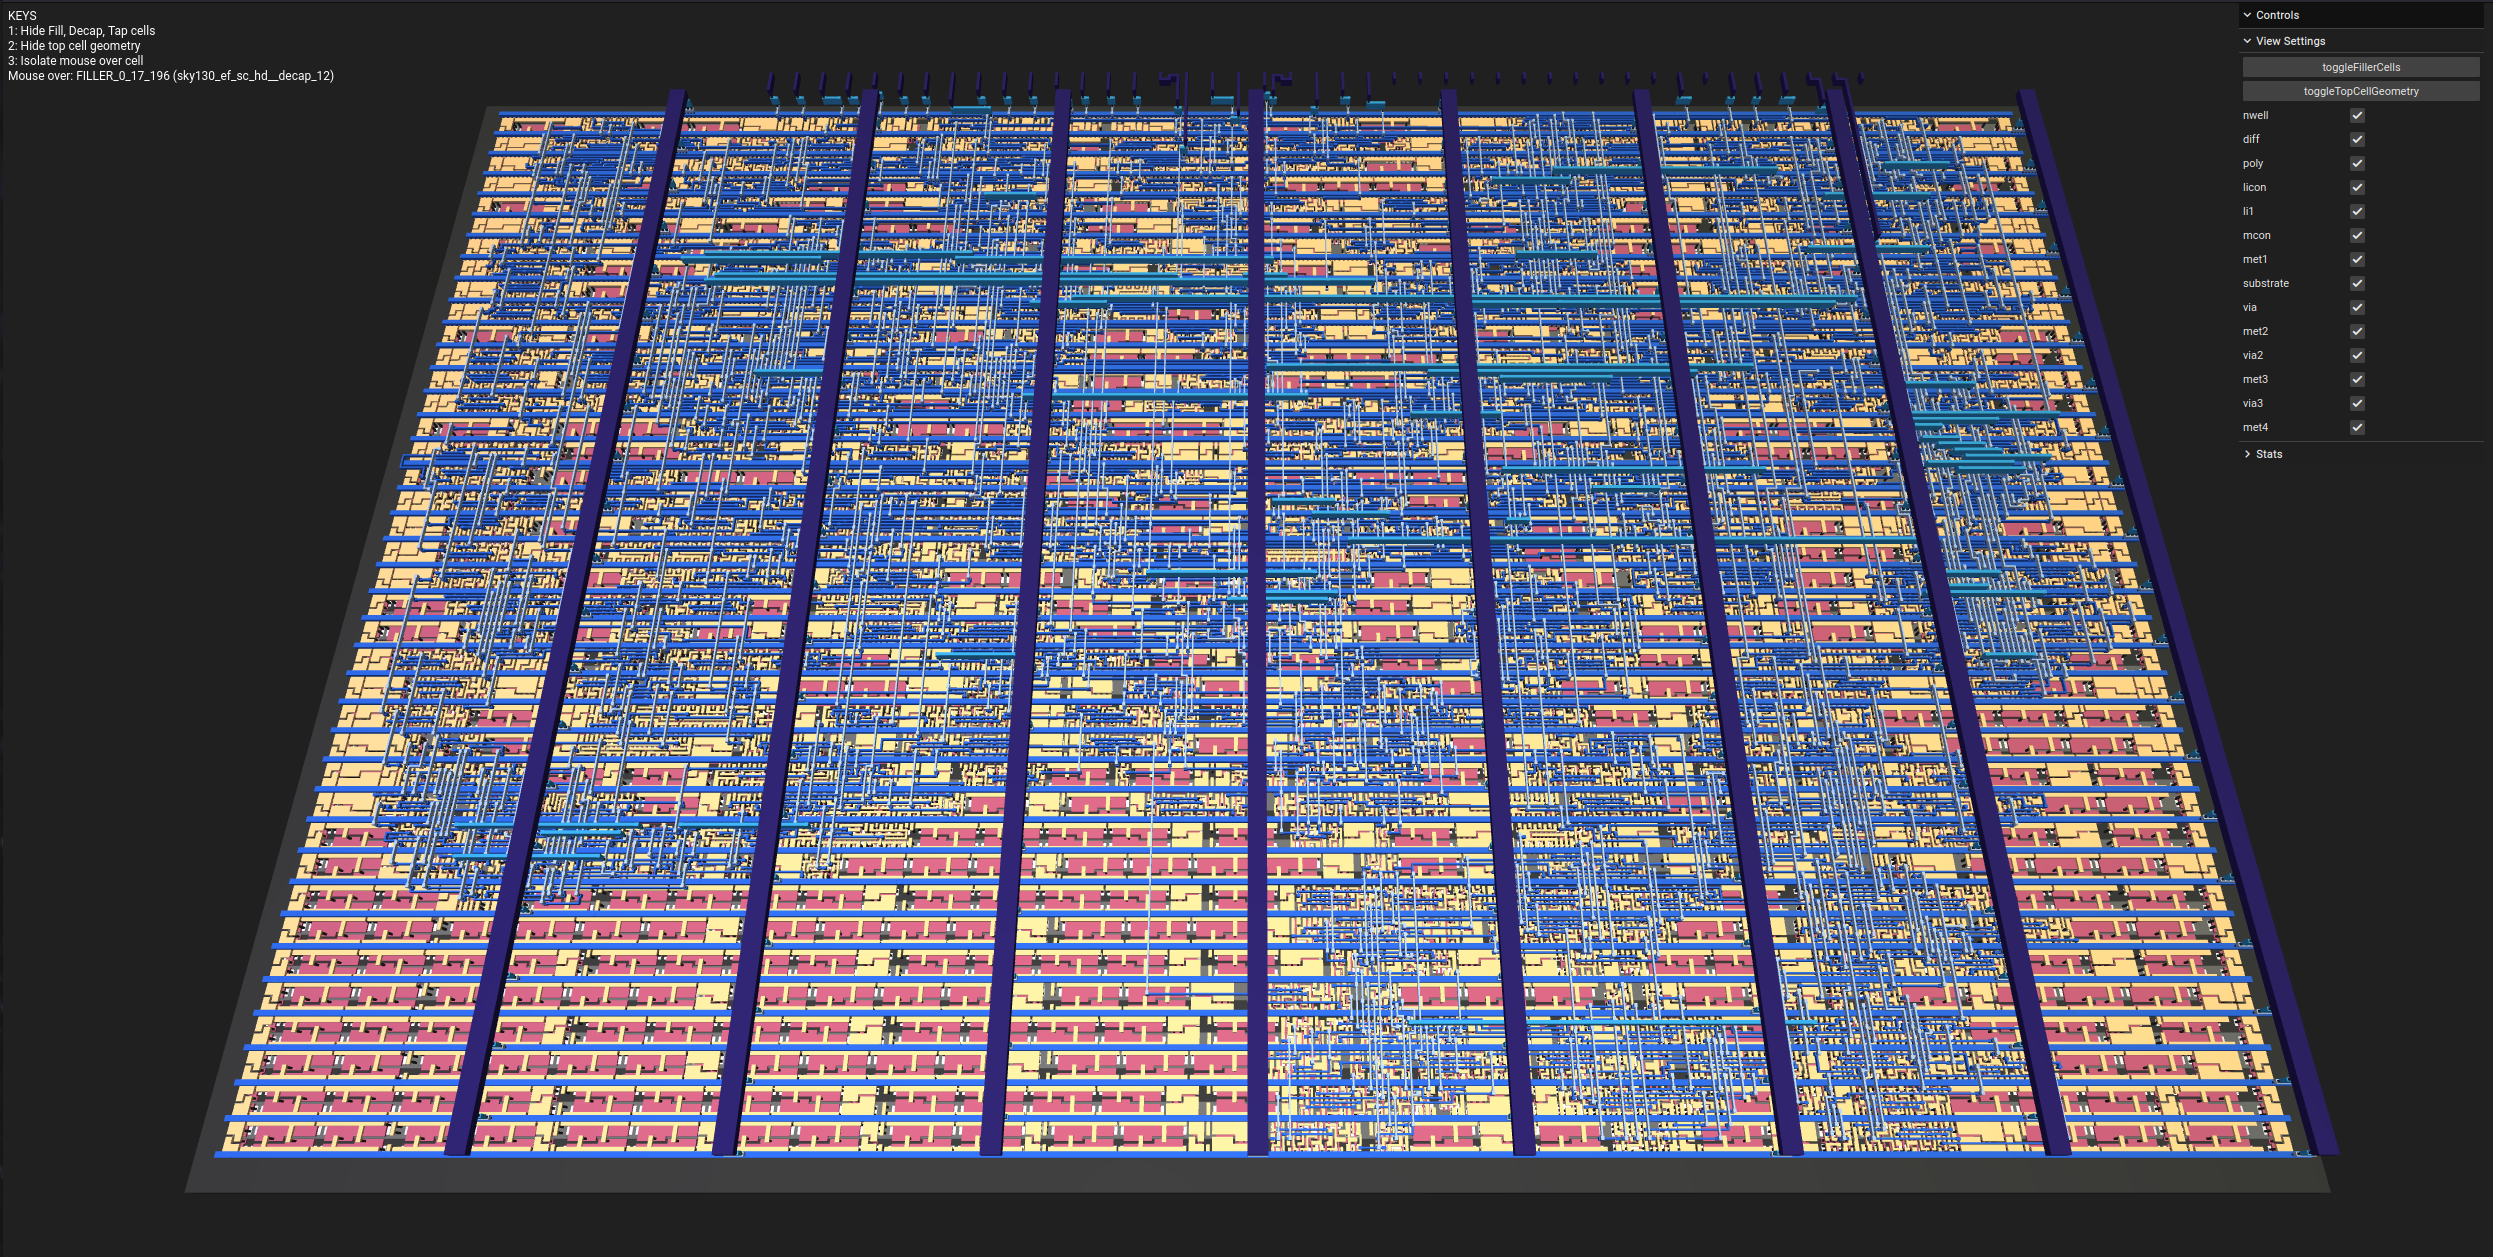
\includegraphics[width=\columnwidth]{./Figs/gh action gds 3d view.png}
\caption{The interactive 3-D viewer.}
\label{fig:interactive_3D_viewer}
\end{figure}
